\documentclass[10pt]{article}
\usepackage[margin=1in]{geometry}
\usepackage[round,authoryear]{natbib}
\usepackage{amsmath,amssymb,booktabs,graphicx}
\usepackage[font=small,labelfont=bf]{caption}
\usepackage{hyperref}
\hypersetup{colorlinks=true,linkcolor=black,citecolor=black,urlcolor=blue}
\setlength{\parskip}{0.35em}

\expandafter\def\csname num@erm_train_end\endcsname{99}
\expandafter\def\csname num@erm_peak_test\endcsname{66.7}
\expandafter\def\csname num@erm_peak_step\endcsname{1{,}500}
\expandafter\def\csname num@erm_test_end\endcsname{63.3}
\expandafter\def\csname num@erm_drop\endcsname{3.3}
\expandafter\def\csname num@erm_val_lo\endcsname{69.3}
\expandafter\def\csname num@erm_val_hi\endcsname{70.3}
\expandafter\def\csname num@erm_vloss_min\endcsname{0.56}
\expandafter\def\csname num@erm_vloss_end\endcsname{1.42}
\expandafter\def\csname num@erm_vloss_min_step\endcsname{1{,}500}
\expandafter\def\csname num@erm_step_val_15000\endcsname{6{,}600}
\expandafter\def\csname num@erm_step_vloss_15000\endcsname{1{,}800}
\expandafter\def\csname num@erm_step_oracle_15000\endcsname{2{,}100}
\expandafter\def\csname num@erm_step_val_30000\endcsname{7{,}100}
\expandafter\def\csname num@erm_step_vloss_30000\endcsname{2{,}100}
\expandafter\def\csname num@erm_step_oracle_30000\endcsname{2{,}200}
\expandafter\def\csname num@acc_ERM_val_750\endcsname{65.8}
\expandafter\def\csname num@acc_ERM_vloss_750\endcsname{65.8}
\expandafter\def\csname num@acc_ERM_last_750\endcsname{66.2}
\expandafter\def\csname num@acc_ERM_oracle_750\endcsname{67.4}
\expandafter\def\csname num@acc_IRM_val_750\endcsname{65.1}
\expandafter\def\csname num@acc_IRM_vloss_750\endcsname{64.3}
\expandafter\def\csname num@acc_IRM_last_750\endcsname{65.3}
\expandafter\def\csname num@acc_IRM_oracle_750\endcsname{67.4}
\expandafter\def\csname num@acc_VREx_val_750\endcsname{65.3}
\expandafter\def\csname num@acc_VREx_vloss_750\endcsname{65.7}
\expandafter\def\csname num@acc_VREx_last_750\endcsname{66.1}
\expandafter\def\csname num@acc_VREx_oracle_750\endcsname{67.3}
\expandafter\def\csname num@acc_GroupDRO_val_750\endcsname{65.7}
\expandafter\def\csname num@acc_GroupDRO_vloss_750\endcsname{65.8}
\expandafter\def\csname num@acc_GroupDRO_last_750\endcsname{66.3}
\expandafter\def\csname num@acc_GroupDRO_oracle_750\endcsname{67.5}
\expandafter\def\csname num@acc_CORAL_val_750\endcsname{65.8}
\expandafter\def\csname num@acc_CORAL_vloss_750\endcsname{65.8}
\expandafter\def\csname num@acc_CORAL_last_750\endcsname{66.2}
\expandafter\def\csname num@acc_CORAL_oracle_750\endcsname{67.4}
\expandafter\def\csname num@acc_SD_val_750\endcsname{65.7}
\expandafter\def\csname num@acc_SD_vloss_750\endcsname{65.8}
\expandafter\def\csname num@acc_SD_last_750\endcsname{66.2}
\expandafter\def\csname num@acc_SD_oracle_750\endcsname{67.5}
\expandafter\def\csname num@acc_Finetune_val_750\endcsname{64.4}
\expandafter\def\csname num@acc_Finetune_vloss_750\endcsname{64.5}
\expandafter\def\csname num@acc_Finetune_last_750\endcsname{64.7}
\expandafter\def\csname num@acc_Finetune_oracle_750\endcsname{66.2}
\expandafter\def\csname num@acc_ER_val_750\endcsname{63.0}
\expandafter\def\csname num@acc_ER_vloss_750\endcsname{62.7}
\expandafter\def\csname num@acc_ER_last_750\endcsname{63.2}
\expandafter\def\csname num@acc_ER_oracle_750\endcsname{64.4}
\expandafter\def\csname num@acc_ER_FF_val_750\endcsname{62.9}
\expandafter\def\csname num@acc_ER_FF_vloss_750\endcsname{62.6}
\expandafter\def\csname num@acc_ER_FF_last_750\endcsname{62.6}
\expandafter\def\csname num@acc_ER_FF_oracle_750\endcsname{63.9}
\expandafter\def\csname num@acc_PDCL_RS_val_750\endcsname{64.5}
\expandafter\def\csname num@acc_PDCL_RS_vloss_750\endcsname{64.5}
\expandafter\def\csname num@acc_PDCL_RS_last_750\endcsname{64.7}
\expandafter\def\csname num@acc_PDCL_RS_oracle_750\endcsname{66.3}
\expandafter\def\csname num@acc_PDCL_val_750\endcsname{64.4}
\expandafter\def\csname num@acc_PDCL_vloss_750\endcsname{64.5}
\expandafter\def\csname num@acc_PDCL_last_750\endcsname{64.6}
\expandafter\def\csname num@acc_PDCL_oracle_750\endcsname{66.2}
\expandafter\def\csname num@d_PDCL_RS_Finetune_val_750\endcsname{$+0.04\pm0.19$}
\expandafter\def\csname num@d_PDCL_RS_ER_val_750\endcsname{$+1.41\pm0.30$}
\expandafter\def\csname num@d_ER_Finetune_val_750\endcsname{$-1.37\pm0.27$}
\expandafter\def\csname num@d_PDCL_PDCL_RS_val_750\endcsname{$-0.04\pm0.18$}
\expandafter\def\csname num@d_ER_FF_ER_val_750\endcsname{$-0.17\pm0.46$}
\expandafter\def\csname num@d_PDCL_RS_ERM_val_750\endcsname{$-1.31\pm0.44$}
\expandafter\def\csname num@d_Finetune_ERM_val_750\endcsname{$-1.34\pm0.44$}
\expandafter\def\csname num@d_IRM_ERM_val_750\endcsname{$-0.68\pm0.35$}
\expandafter\def\csname num@d_VREx_ERM_val_750\endcsname{$-0.42\pm0.31$}
\expandafter\def\csname num@d_GroupDRO_ERM_val_750\endcsname{$-0.11\pm0.30$}
\expandafter\def\csname num@d_CORAL_ERM_val_750\endcsname{$+0.05\pm0.15$}
\expandafter\def\csname num@d_SD_ERM_val_750\endcsname{$-0.04\pm0.19$}
\expandafter\def\csname num@d_PDCL_RS_Finetune_vloss_750\endcsname{$+0.01\pm0.07$}
\expandafter\def\csname num@d_PDCL_RS_ER_vloss_750\endcsname{$+1.80\pm0.37$}
\expandafter\def\csname num@d_ER_Finetune_vloss_750\endcsname{$-1.79\pm0.36$}
\expandafter\def\csname num@d_PDCL_PDCL_RS_vloss_750\endcsname{$-0.06\pm0.06$}
\expandafter\def\csname num@d_ER_FF_ER_vloss_750\endcsname{$-0.17\pm0.40$}
\expandafter\def\csname num@d_PDCL_RS_ERM_vloss_750\endcsname{$-1.22\pm0.33$}
\expandafter\def\csname num@d_Finetune_ERM_vloss_750\endcsname{$-1.23\pm0.34$}
\expandafter\def\csname num@d_IRM_ERM_vloss_750\endcsname{$-1.43\pm0.38$}
\expandafter\def\csname num@d_VREx_ERM_vloss_750\endcsname{$-0.09\pm0.23$}
\expandafter\def\csname num@d_GroupDRO_ERM_vloss_750\endcsname{$+0.03\pm0.16$}
\expandafter\def\csname num@d_CORAL_ERM_vloss_750\endcsname{$+0.06\pm0.14$}
\expandafter\def\csname num@d_SD_ERM_vloss_750\endcsname{$+0.09\pm0.12$}
\expandafter\def\csname num@d_rule_750\endcsname{$-0.00\pm0.17$}
\expandafter\def\csname num@acc_ERM_val_1500\endcsname{66.3}
\expandafter\def\csname num@acc_ERM_vloss_1500\endcsname{66.5}
\expandafter\def\csname num@acc_ERM_last_1500\endcsname{66.7}
\expandafter\def\csname num@acc_ERM_oracle_1500\endcsname{68.4}
\expandafter\def\csname num@acc_IRM_val_1500\endcsname{65.1}
\expandafter\def\csname num@acc_IRM_vloss_1500\endcsname{64.4}
\expandafter\def\csname num@acc_IRM_last_1500\endcsname{63.9}
\expandafter\def\csname num@acc_IRM_oracle_1500\endcsname{67.7}
\expandafter\def\csname num@acc_VREx_val_1500\endcsname{66.8}
\expandafter\def\csname num@acc_VREx_vloss_1500\endcsname{66.6}
\expandafter\def\csname num@acc_VREx_last_1500\endcsname{66.9}
\expandafter\def\csname num@acc_VREx_oracle_1500\endcsname{68.5}
\expandafter\def\csname num@acc_GroupDRO_val_1500\endcsname{66.2}
\expandafter\def\csname num@acc_GroupDRO_vloss_1500\endcsname{66.6}
\expandafter\def\csname num@acc_GroupDRO_last_1500\endcsname{66.8}
\expandafter\def\csname num@acc_GroupDRO_oracle_1500\endcsname{68.5}
\expandafter\def\csname num@acc_CORAL_val_1500\endcsname{66.2}
\expandafter\def\csname num@acc_CORAL_vloss_1500\endcsname{66.7}
\expandafter\def\csname num@acc_CORAL_last_1500\endcsname{66.8}
\expandafter\def\csname num@acc_CORAL_oracle_1500\endcsname{68.4}
\expandafter\def\csname num@acc_SD_val_1500\endcsname{66.5}
\expandafter\def\csname num@acc_SD_vloss_1500\endcsname{66.6}
\expandafter\def\csname num@acc_SD_last_1500\endcsname{66.7}
\expandafter\def\csname num@acc_SD_oracle_1500\endcsname{68.4}
\expandafter\def\csname num@acc_Finetune_val_1500\endcsname{65.4}
\expandafter\def\csname num@acc_Finetune_vloss_1500\endcsname{65.9}
\expandafter\def\csname num@acc_Finetune_last_1500\endcsname{65.8}
\expandafter\def\csname num@acc_Finetune_oracle_1500\endcsname{67.5}
\expandafter\def\csname num@acc_ER_val_1500\endcsname{64.1}
\expandafter\def\csname num@acc_ER_vloss_1500\endcsname{63.5}
\expandafter\def\csname num@acc_ER_last_1500\endcsname{64.0}
\expandafter\def\csname num@acc_ER_oracle_1500\endcsname{65.8}
\expandafter\def\csname num@acc_ER_FF_val_1500\endcsname{63.6}
\expandafter\def\csname num@acc_ER_FF_vloss_1500\endcsname{62.8}
\expandafter\def\csname num@acc_ER_FF_last_1500\endcsname{63.9}
\expandafter\def\csname num@acc_ER_FF_oracle_1500\endcsname{65.2}
\expandafter\def\csname num@acc_PDCL_RS_val_1500\endcsname{65.6}
\expandafter\def\csname num@acc_PDCL_RS_vloss_1500\endcsname{66.0}
\expandafter\def\csname num@acc_PDCL_RS_last_1500\endcsname{65.9}
\expandafter\def\csname num@acc_PDCL_RS_oracle_1500\endcsname{67.6}
\expandafter\def\csname num@acc_PDCL_val_1500\endcsname{65.8}
\expandafter\def\csname num@acc_PDCL_vloss_1500\endcsname{65.7}
\expandafter\def\csname num@acc_PDCL_last_1500\endcsname{65.9}
\expandafter\def\csname num@acc_PDCL_oracle_1500\endcsname{67.7}
\expandafter\def\csname num@d_PDCL_RS_Finetune_val_1500\endcsname{$+0.11\pm0.26$}
\expandafter\def\csname num@d_PDCL_RS_ER_val_1500\endcsname{$+1.46\pm0.39$}
\expandafter\def\csname num@d_ER_Finetune_val_1500\endcsname{$-1.35\pm0.40$}
\expandafter\def\csname num@d_PDCL_PDCL_RS_val_1500\endcsname{$+0.25\pm0.23$}
\expandafter\def\csname num@d_ER_FF_ER_val_1500\endcsname{$-0.54\pm0.36$}
\expandafter\def\csname num@d_PDCL_RS_ERM_val_1500\endcsname{$-0.79\pm0.37$}
\expandafter\def\csname num@d_Finetune_ERM_val_1500\endcsname{$-0.90\pm0.29$}
\expandafter\def\csname num@d_IRM_ERM_val_1500\endcsname{$-1.22\pm0.31$}
\expandafter\def\csname num@d_VREx_ERM_val_1500\endcsname{$+0.41\pm0.15$}
\expandafter\def\csname num@d_GroupDRO_ERM_val_1500\endcsname{$-0.10\pm0.26$}
\expandafter\def\csname num@d_CORAL_ERM_val_1500\endcsname{$-0.10\pm0.12$}
\expandafter\def\csname num@d_SD_ERM_val_1500\endcsname{$+0.15\pm0.16$}
\expandafter\def\csname num@d_PDCL_RS_Finetune_vloss_1500\endcsname{$+0.10\pm0.11$}
\expandafter\def\csname num@d_PDCL_RS_ER_vloss_1500\endcsname{$+2.52\pm0.32$}
\expandafter\def\csname num@d_ER_Finetune_vloss_1500\endcsname{$-2.41\pm0.34$}
\expandafter\def\csname num@d_PDCL_PDCL_RS_vloss_1500\endcsname{$-0.34\pm0.19$}
\expandafter\def\csname num@d_ER_FF_ER_vloss_1500\endcsname{$-0.70\pm0.26$}
\expandafter\def\csname num@d_PDCL_RS_ERM_vloss_1500\endcsname{$-0.48\pm0.24$}
\expandafter\def\csname num@d_Finetune_ERM_vloss_1500\endcsname{$-0.58\pm0.18$}
\expandafter\def\csname num@d_IRM_ERM_vloss_1500\endcsname{$-2.12\pm0.31$}
\expandafter\def\csname num@d_VREx_ERM_vloss_1500\endcsname{$+0.10\pm0.11$}
\expandafter\def\csname num@d_GroupDRO_ERM_vloss_1500\endcsname{$+0.07\pm0.13$}
\expandafter\def\csname num@d_CORAL_ERM_vloss_1500\endcsname{$+0.20\pm0.07$}
\expandafter\def\csname num@d_SD_ERM_vloss_1500\endcsname{$+0.07\pm0.12$}
\expandafter\def\csname num@d_rule_1500\endcsname{$+0.16\pm0.13$}
\expandafter\def\csname num@acc_ERM_val_3000\endcsname{66.6}
\expandafter\def\csname num@acc_ERM_vloss_3000\endcsname{66.6}
\expandafter\def\csname num@acc_ERM_last_3000\endcsname{66.3}
\expandafter\def\csname num@acc_ERM_oracle_3000\endcsname{68.5}
\expandafter\def\csname num@acc_IRM_val_3000\endcsname{64.9}
\expandafter\def\csname num@acc_IRM_vloss_3000\endcsname{64.6}
\expandafter\def\csname num@acc_IRM_last_3000\endcsname{63.8}
\expandafter\def\csname num@acc_IRM_oracle_3000\endcsname{67.4}
\expandafter\def\csname num@acc_VREx_val_3000\endcsname{67.0}
\expandafter\def\csname num@acc_VREx_vloss_3000\endcsname{66.6}
\expandafter\def\csname num@acc_VREx_last_3000\endcsname{66.6}
\expandafter\def\csname num@acc_VREx_oracle_3000\endcsname{68.5}
\expandafter\def\csname num@acc_GroupDRO_val_3000\endcsname{66.9}
\expandafter\def\csname num@acc_GroupDRO_vloss_3000\endcsname{66.9}
\expandafter\def\csname num@acc_GroupDRO_last_3000\endcsname{66.4}
\expandafter\def\csname num@acc_GroupDRO_oracle_3000\endcsname{68.6}
\expandafter\def\csname num@acc_CORAL_val_3000\endcsname{66.8}
\expandafter\def\csname num@acc_CORAL_vloss_3000\endcsname{66.6}
\expandafter\def\csname num@acc_CORAL_last_3000\endcsname{66.2}
\expandafter\def\csname num@acc_CORAL_oracle_3000\endcsname{68.5}
\expandafter\def\csname num@acc_SD_val_3000\endcsname{66.8}
\expandafter\def\csname num@acc_SD_vloss_3000\endcsname{66.4}
\expandafter\def\csname num@acc_SD_last_3000\endcsname{66.3}
\expandafter\def\csname num@acc_SD_oracle_3000\endcsname{68.4}
\expandafter\def\csname num@acc_Finetune_val_3000\endcsname{65.4}
\expandafter\def\csname num@acc_Finetune_vloss_3000\endcsname{65.8}
\expandafter\def\csname num@acc_Finetune_last_3000\endcsname{65.6}
\expandafter\def\csname num@acc_Finetune_oracle_3000\endcsname{67.3}
\expandafter\def\csname num@acc_ER_val_3000\endcsname{64.3}
\expandafter\def\csname num@acc_ER_vloss_3000\endcsname{64.1}
\expandafter\def\csname num@acc_ER_last_3000\endcsname{64.4}
\expandafter\def\csname num@acc_ER_oracle_3000\endcsname{65.9}
\expandafter\def\csname num@acc_ER_FF_val_3000\endcsname{63.7}
\expandafter\def\csname num@acc_ER_FF_vloss_3000\endcsname{63.1}
\expandafter\def\csname num@acc_ER_FF_last_3000\endcsname{63.9}
\expandafter\def\csname num@acc_ER_FF_oracle_3000\endcsname{65.4}
\expandafter\def\csname num@acc_PDCL_RS_val_3000\endcsname{65.9}
\expandafter\def\csname num@acc_PDCL_RS_vloss_3000\endcsname{66.0}
\expandafter\def\csname num@acc_PDCL_RS_last_3000\endcsname{65.7}
\expandafter\def\csname num@acc_PDCL_RS_oracle_3000\endcsname{67.4}
\expandafter\def\csname num@acc_PDCL_val_3000\endcsname{65.7}
\expandafter\def\csname num@acc_PDCL_vloss_3000\endcsname{65.7}
\expandafter\def\csname num@acc_PDCL_last_3000\endcsname{65.7}
\expandafter\def\csname num@acc_PDCL_oracle_3000\endcsname{67.5}
\expandafter\def\csname num@d_PDCL_RS_Finetune_val_3000\endcsname{$+0.49\pm0.19$}
\expandafter\def\csname num@d_PDCL_RS_ER_val_3000\endcsname{$+1.58\pm0.25$}
\expandafter\def\csname num@d_ER_Finetune_val_3000\endcsname{$-1.09\pm0.33$}
\expandafter\def\csname num@d_PDCL_PDCL_RS_val_3000\endcsname{$-0.14\pm0.22$}
\expandafter\def\csname num@d_ER_FF_ER_val_3000\endcsname{$-0.59\pm0.36$}
\expandafter\def\csname num@d_PDCL_RS_ERM_val_3000\endcsname{$-0.76\pm0.32$}
\expandafter\def\csname num@d_Finetune_ERM_val_3000\endcsname{$-1.25\pm0.32$}
\expandafter\def\csname num@d_IRM_ERM_val_3000\endcsname{$-1.75\pm0.34$}
\expandafter\def\csname num@d_VREx_ERM_val_3000\endcsname{$+0.34\pm0.16$}
\expandafter\def\csname num@d_GroupDRO_ERM_val_3000\endcsname{$+0.23\pm0.18$}
\expandafter\def\csname num@d_CORAL_ERM_val_3000\endcsname{$+0.12\pm0.16$}
\expandafter\def\csname num@d_SD_ERM_val_3000\endcsname{$+0.20\pm0.12$}
\expandafter\def\csname num@d_PDCL_RS_Finetune_vloss_3000\endcsname{$+0.20\pm0.18$}
\expandafter\def\csname num@d_PDCL_RS_ER_vloss_3000\endcsname{$+1.93\pm0.34$}
\expandafter\def\csname num@d_ER_Finetune_vloss_3000\endcsname{$-1.73\pm0.43$}
\expandafter\def\csname num@d_PDCL_PDCL_RS_vloss_3000\endcsname{$-0.29\pm0.23$}
\expandafter\def\csname num@d_ER_FF_ER_vloss_3000\endcsname{$-0.99\pm0.30$}
\expandafter\def\csname num@d_PDCL_RS_ERM_vloss_3000\endcsname{$-0.59\pm0.25$}
\expandafter\def\csname num@d_Finetune_ERM_vloss_3000\endcsname{$-0.79\pm0.28$}
\expandafter\def\csname num@d_IRM_ERM_vloss_3000\endcsname{$-1.98\pm0.33$}
\expandafter\def\csname num@d_VREx_ERM_vloss_3000\endcsname{$+0.00\pm0.19$}
\expandafter\def\csname num@d_GroupDRO_ERM_vloss_3000\endcsname{$+0.29\pm0.14$}
\expandafter\def\csname num@d_CORAL_ERM_vloss_3000\endcsname{$-0.06\pm0.07$}
\expandafter\def\csname num@d_SD_ERM_vloss_3000\endcsname{$-0.24\pm0.12$}
\expandafter\def\csname num@d_rule_3000\endcsname{$-0.03\pm0.17$}
\expandafter\def\csname num@acc_ERM_val_6000\endcsname{65.9}
\expandafter\def\csname num@acc_ERM_vloss_6000\endcsname{66.3}
\expandafter\def\csname num@acc_ERM_last_6000\endcsname{64.7}
\expandafter\def\csname num@acc_ERM_oracle_6000\endcsname{68.3}
\expandafter\def\csname num@acc_IRM_val_6000\endcsname{64.7}
\expandafter\def\csname num@acc_IRM_vloss_6000\endcsname{64.7}
\expandafter\def\csname num@acc_IRM_last_6000\endcsname{64.1}
\expandafter\def\csname num@acc_IRM_oracle_6000\endcsname{67.3}
\expandafter\def\csname num@acc_VREx_val_6000\endcsname{66.2}
\expandafter\def\csname num@acc_VREx_vloss_6000\endcsname{66.4}
\expandafter\def\csname num@acc_VREx_last_6000\endcsname{65.3}
\expandafter\def\csname num@acc_VREx_oracle_6000\endcsname{68.4}
\expandafter\def\csname num@acc_GroupDRO_val_6000\endcsname{65.9}
\expandafter\def\csname num@acc_GroupDRO_vloss_6000\endcsname{66.6}
\expandafter\def\csname num@acc_GroupDRO_last_6000\endcsname{65.0}
\expandafter\def\csname num@acc_GroupDRO_oracle_6000\endcsname{68.5}
\expandafter\def\csname num@acc_CORAL_val_6000\endcsname{65.8}
\expandafter\def\csname num@acc_CORAL_vloss_6000\endcsname{66.3}
\expandafter\def\csname num@acc_CORAL_last_6000\endcsname{64.7}
\expandafter\def\csname num@acc_CORAL_oracle_6000\endcsname{68.3}
\expandafter\def\csname num@acc_SD_val_6000\endcsname{65.7}
\expandafter\def\csname num@acc_SD_vloss_6000\endcsname{66.2}
\expandafter\def\csname num@acc_SD_last_6000\endcsname{64.2}
\expandafter\def\csname num@acc_SD_oracle_6000\endcsname{68.2}
\expandafter\def\csname num@acc_Finetune_val_6000\endcsname{65.1}
\expandafter\def\csname num@acc_Finetune_vloss_6000\endcsname{65.2}
\expandafter\def\csname num@acc_Finetune_last_6000\endcsname{64.6}
\expandafter\def\csname num@acc_Finetune_oracle_6000\endcsname{66.3}
\expandafter\def\csname num@acc_ER_val_6000\endcsname{63.9}
\expandafter\def\csname num@acc_ER_vloss_6000\endcsname{64.1}
\expandafter\def\csname num@acc_ER_last_6000\endcsname{63.4}
\expandafter\def\csname num@acc_ER_oracle_6000\endcsname{65.1}
\expandafter\def\csname num@acc_ER_FF_val_6000\endcsname{63.4}
\expandafter\def\csname num@acc_ER_FF_vloss_6000\endcsname{63.7}
\expandafter\def\csname num@acc_ER_FF_last_6000\endcsname{63.4}
\expandafter\def\csname num@acc_ER_FF_oracle_6000\endcsname{64.8}
\expandafter\def\csname num@acc_PDCL_RS_val_6000\endcsname{65.0}
\expandafter\def\csname num@acc_PDCL_RS_vloss_6000\endcsname{65.4}
\expandafter\def\csname num@acc_PDCL_RS_last_6000\endcsname{64.5}
\expandafter\def\csname num@acc_PDCL_RS_oracle_6000\endcsname{66.2}
\expandafter\def\csname num@acc_PDCL_val_6000\endcsname{64.9}
\expandafter\def\csname num@acc_PDCL_vloss_6000\endcsname{65.0}
\expandafter\def\csname num@acc_PDCL_last_6000\endcsname{64.4}
\expandafter\def\csname num@acc_PDCL_oracle_6000\endcsname{66.1}
\expandafter\def\csname num@d_PDCL_RS_Finetune_val_6000\endcsname{$-0.14\pm0.24$}
\expandafter\def\csname num@d_PDCL_RS_ER_val_6000\endcsname{$+1.06\pm0.23$}
\expandafter\def\csname num@d_ER_Finetune_val_6000\endcsname{$-1.20\pm0.28$}
\expandafter\def\csname num@d_PDCL_PDCL_RS_val_6000\endcsname{$-0.07\pm0.20$}
\expandafter\def\csname num@d_ER_FF_ER_val_6000\endcsname{$-0.54\pm0.24$}
\expandafter\def\csname num@d_PDCL_RS_ERM_val_6000\endcsname{$-0.94\pm0.33$}
\expandafter\def\csname num@d_Finetune_ERM_val_6000\endcsname{$-0.81\pm0.36$}
\expandafter\def\csname num@d_IRM_ERM_val_6000\endcsname{$-1.25\pm0.42$}
\expandafter\def\csname num@d_VREx_ERM_val_6000\endcsname{$+0.29\pm0.28$}
\expandafter\def\csname num@d_GroupDRO_ERM_val_6000\endcsname{$+0.01\pm0.24$}
\expandafter\def\csname num@d_CORAL_ERM_val_6000\endcsname{$-0.11\pm0.25$}
\expandafter\def\csname num@d_SD_ERM_val_6000\endcsname{$-0.20\pm0.36$}
\expandafter\def\csname num@d_PDCL_RS_Finetune_vloss_6000\endcsname{$+0.19\pm0.15$}
\expandafter\def\csname num@d_PDCL_RS_ER_vloss_6000\endcsname{$+1.30\pm0.25$}
\expandafter\def\csname num@d_ER_Finetune_vloss_6000\endcsname{$-1.11\pm0.26$}
\expandafter\def\csname num@d_PDCL_PDCL_RS_vloss_6000\endcsname{$-0.35\pm0.13$}
\expandafter\def\csname num@d_ER_FF_ER_vloss_6000\endcsname{$-0.42\pm0.24$}
\expandafter\def\csname num@d_PDCL_RS_ERM_vloss_6000\endcsname{$-0.93\pm0.15$}
\expandafter\def\csname num@d_Finetune_ERM_vloss_6000\endcsname{$-1.12\pm0.18$}
\expandafter\def\csname num@d_IRM_ERM_vloss_6000\endcsname{$-1.59\pm0.23$}
\expandafter\def\csname num@d_VREx_ERM_vloss_6000\endcsname{$+0.13\pm0.24$}
\expandafter\def\csname num@d_GroupDRO_ERM_vloss_6000\endcsname{$+0.31\pm0.16$}
\expandafter\def\csname num@d_CORAL_ERM_vloss_6000\endcsname{$+0.04\pm0.11$}
\expandafter\def\csname num@d_SD_ERM_vloss_6000\endcsname{$-0.13\pm0.21$}
\expandafter\def\csname num@d_rule_6000\endcsname{$+0.38\pm0.26$}
\expandafter\def\csname num@acc_ERM_val_15000\endcsname{64.8}
\expandafter\def\csname num@acc_ERM_vloss_15000\endcsname{66.4}
\expandafter\def\csname num@acc_ERM_last_15000\endcsname{63.3}
\expandafter\def\csname num@acc_ERM_oracle_15000\endcsname{67.7}
\expandafter\def\csname num@acc_IRM_val_15000\endcsname{64.4}
\expandafter\def\csname num@acc_IRM_vloss_15000\endcsname{64.3}
\expandafter\def\csname num@acc_IRM_last_15000\endcsname{64.1}
\expandafter\def\csname num@acc_IRM_oracle_15000\endcsname{67.5}
\expandafter\def\csname num@acc_VREx_val_15000\endcsname{65.6}
\expandafter\def\csname num@acc_VREx_vloss_15000\endcsname{66.2}
\expandafter\def\csname num@acc_VREx_last_15000\endcsname{63.6}
\expandafter\def\csname num@acc_VREx_oracle_15000\endcsname{68.1}
\expandafter\def\csname num@acc_GroupDRO_val_15000\endcsname{65.5}
\expandafter\def\csname num@acc_GroupDRO_vloss_15000\endcsname{66.6}
\expandafter\def\csname num@acc_GroupDRO_last_15000\endcsname{63.6}
\expandafter\def\csname num@acc_GroupDRO_oracle_15000\endcsname{67.9}
\expandafter\def\csname num@acc_CORAL_val_15000\endcsname{65.7}
\expandafter\def\csname num@acc_CORAL_vloss_15000\endcsname{66.4}
\expandafter\def\csname num@acc_CORAL_last_15000\endcsname{63.2}
\expandafter\def\csname num@acc_CORAL_oracle_15000\endcsname{67.6}
\expandafter\def\csname num@acc_SD_val_15000\endcsname{65.0}
\expandafter\def\csname num@acc_SD_vloss_15000\endcsname{66.2}
\expandafter\def\csname num@acc_SD_last_15000\endcsname{61.6}
\expandafter\def\csname num@acc_SD_oracle_15000\endcsname{67.7}
\expandafter\def\csname num@acc_Finetune_val_15000\endcsname{62.5}
\expandafter\def\csname num@acc_Finetune_vloss_15000\endcsname{62.9}
\expandafter\def\csname num@acc_Finetune_last_15000\endcsname{62.4}
\expandafter\def\csname num@acc_Finetune_oracle_15000\endcsname{63.9}
\expandafter\def\csname num@acc_ER_val_15000\endcsname{62.4}
\expandafter\def\csname num@acc_ER_vloss_15000\endcsname{62.6}
\expandafter\def\csname num@acc_ER_last_15000\endcsname{62.4}
\expandafter\def\csname num@acc_ER_oracle_15000\endcsname{63.5}
\expandafter\def\csname num@acc_ER_FF_val_15000\endcsname{62.0}
\expandafter\def\csname num@acc_ER_FF_vloss_15000\endcsname{62.2}
\expandafter\def\csname num@acc_ER_FF_last_15000\endcsname{62.1}
\expandafter\def\csname num@acc_ER_FF_oracle_15000\endcsname{63.3}
\expandafter\def\csname num@acc_PDCL_RS_val_15000\endcsname{62.7}
\expandafter\def\csname num@acc_PDCL_RS_vloss_15000\endcsname{62.6}
\expandafter\def\csname num@acc_PDCL_RS_last_15000\endcsname{62.5}
\expandafter\def\csname num@acc_PDCL_RS_oracle_15000\endcsname{64.0}
\expandafter\def\csname num@acc_PDCL_val_15000\endcsname{62.4}
\expandafter\def\csname num@acc_PDCL_vloss_15000\endcsname{62.4}
\expandafter\def\csname num@acc_PDCL_last_15000\endcsname{62.4}
\expandafter\def\csname num@acc_PDCL_oracle_15000\endcsname{63.6}
\expandafter\def\csname num@d_PDCL_RS_Finetune_val_15000\endcsname{$+0.17\pm0.37$}
\expandafter\def\csname num@d_PDCL_RS_ER_val_15000\endcsname{$+0.26\pm0.37$}
\expandafter\def\csname num@d_ER_Finetune_val_15000\endcsname{$-0.08\pm0.23$}
\expandafter\def\csname num@d_PDCL_PDCL_RS_val_15000\endcsname{$-0.29\pm0.41$}
\expandafter\def\csname num@d_ER_FF_ER_val_15000\endcsname{$-0.37\pm0.21$}
\expandafter\def\csname num@d_PDCL_RS_ERM_val_15000\endcsname{$-2.13\pm0.31$}
\expandafter\def\csname num@d_Finetune_ERM_val_15000\endcsname{$-2.31\pm0.24$}
\expandafter\def\csname num@d_IRM_ERM_val_15000\endcsname{$-0.45\pm0.30$}
\expandafter\def\csname num@d_VREx_ERM_val_15000\endcsname{$+0.77\pm0.26$}
\expandafter\def\csname num@d_GroupDRO_ERM_val_15000\endcsname{$+0.74\pm0.25$}
\expandafter\def\csname num@d_CORAL_ERM_val_15000\endcsname{$+0.86\pm0.20$}
\expandafter\def\csname num@d_SD_ERM_val_15000\endcsname{$+0.24\pm0.31$}
\expandafter\def\csname num@d_PDCL_RS_Finetune_vloss_15000\endcsname{$-0.22\pm0.16$}
\expandafter\def\csname num@d_PDCL_RS_ER_vloss_15000\endcsname{$+0.08\pm0.26$}
\expandafter\def\csname num@d_ER_Finetune_vloss_15000\endcsname{$-0.30\pm0.20$}
\expandafter\def\csname num@d_PDCL_PDCL_RS_vloss_15000\endcsname{$-0.23\pm0.32$}
\expandafter\def\csname num@d_ER_FF_ER_vloss_15000\endcsname{$-0.36\pm0.20$}
\expandafter\def\csname num@d_PDCL_RS_ERM_vloss_15000\endcsname{$-3.77\pm0.19$}
\expandafter\def\csname num@d_Finetune_ERM_vloss_15000\endcsname{$-3.55\pm0.22$}
\expandafter\def\csname num@d_IRM_ERM_vloss_15000\endcsname{$-2.14\pm0.36$}
\expandafter\def\csname num@d_VREx_ERM_vloss_15000\endcsname{$-0.18\pm0.25$}
\expandafter\def\csname num@d_GroupDRO_ERM_vloss_15000\endcsname{$+0.16\pm0.10$}
\expandafter\def\csname num@d_CORAL_ERM_vloss_15000\endcsname{$+0.03\pm0.05$}
\expandafter\def\csname num@d_SD_ERM_vloss_15000\endcsname{$-0.21\pm0.17$}
\expandafter\def\csname num@d_rule_15000\endcsname{$+1.61\pm0.16$}
\expandafter\def\csname num@acc_ERM_val_30000\endcsname{65.2}
\expandafter\def\csname num@acc_ERM_vloss_30000\endcsname{66.5}
\expandafter\def\csname num@acc_ERM_last_30000\endcsname{62.6}
\expandafter\def\csname num@acc_ERM_oracle_30000\endcsname{67.5}
\expandafter\def\csname num@acc_Finetune_val_30000\endcsname{61.7}
\expandafter\def\csname num@acc_Finetune_vloss_30000\endcsname{61.6}
\expandafter\def\csname num@acc_Finetune_last_30000\endcsname{61.7}
\expandafter\def\csname num@acc_Finetune_oracle_30000\endcsname{62.9}
\expandafter\def\csname num@acc_ER_val_30000\endcsname{61.4}
\expandafter\def\csname num@acc_ER_vloss_30000\endcsname{61.2}
\expandafter\def\csname num@acc_ER_last_30000\endcsname{61.5}
\expandafter\def\csname num@acc_ER_oracle_30000\endcsname{62.6}
\expandafter\def\csname num@acc_ER_FF_val_30000\endcsname{61.5}
\expandafter\def\csname num@acc_ER_FF_vloss_30000\endcsname{61.3}
\expandafter\def\csname num@acc_ER_FF_last_30000\endcsname{61.9}
\expandafter\def\csname num@acc_ER_FF_oracle_30000\endcsname{62.8}
\expandafter\def\csname num@acc_PDCL_RS_val_30000\endcsname{61.7}
\expandafter\def\csname num@acc_PDCL_RS_vloss_30000\endcsname{61.8}
\expandafter\def\csname num@acc_PDCL_RS_last_30000\endcsname{61.8}
\expandafter\def\csname num@acc_PDCL_RS_oracle_30000\endcsname{62.9}
\expandafter\def\csname num@acc_PDCL_val_30000\endcsname{61.4}
\expandafter\def\csname num@acc_PDCL_vloss_30000\endcsname{61.5}
\expandafter\def\csname num@acc_PDCL_last_30000\endcsname{61.6}
\expandafter\def\csname num@acc_PDCL_oracle_30000\endcsname{62.6}
\expandafter\def\csname num@d_PDCL_RS_Finetune_val_30000\endcsname{$+0.04\pm0.54$}
\expandafter\def\csname num@d_PDCL_RS_ER_val_30000\endcsname{$+0.32\pm0.53$}
\expandafter\def\csname num@d_ER_Finetune_val_30000\endcsname{$-0.29\pm0.63$}
\expandafter\def\csname num@d_PDCL_PDCL_RS_val_30000\endcsname{$-0.31\pm0.35$}
\expandafter\def\csname num@d_ER_FF_ER_val_30000\endcsname{$+0.03\pm0.57$}
\expandafter\def\csname num@d_PDCL_RS_ERM_val_30000\endcsname{$-3.49\pm0.53$}
\expandafter\def\csname num@d_Finetune_ERM_val_30000\endcsname{$-3.52\pm0.04$}
\expandafter\def\csname num@d_PDCL_RS_Finetune_vloss_30000\endcsname{$+0.19\pm0.39$}
\expandafter\def\csname num@d_PDCL_RS_ER_vloss_30000\endcsname{$+0.62\pm0.22$}
\expandafter\def\csname num@d_ER_Finetune_vloss_30000\endcsname{$-0.43\pm0.50$}
\expandafter\def\csname num@d_PDCL_PDCL_RS_vloss_30000\endcsname{$-0.28\pm0.29$}
\expandafter\def\csname num@d_ER_FF_ER_vloss_30000\endcsname{$+0.10\pm0.30$}
\expandafter\def\csname num@d_PDCL_RS_ERM_vloss_30000\endcsname{$-4.72\pm0.24$}
\expandafter\def\csname num@d_Finetune_ERM_vloss_30000\endcsname{$-4.92\pm0.46$}
\expandafter\def\csname num@d_rule_30000\endcsname{$+1.28\pm0.55$}
\expandafter\def\csname num@train_Finetune_3000\endcsname{78}
\expandafter\def\csname num@val_Finetune_3000\endcsname{70}
\expandafter\def\csname num@mem_Finetune_3000\endcsname{0.000}
\expandafter\def\csname num@eps_Finetune_3000\endcsname{0.000}
\expandafter\def\csname num@dual_Finetune_3000\endcsname{0.000}
\expandafter\def\csname num@train_ER_3000\endcsname{81}
\expandafter\def\csname num@val_ER_3000\endcsname{69}
\expandafter\def\csname num@mem_ER_3000\endcsname{0.033}
\expandafter\def\csname num@eps_ER_3000\endcsname{0.521}
\expandafter\def\csname num@dual_ER_3000\endcsname{0.000}
\expandafter\def\csname num@train_PDCL_RS_3000\endcsname{78}
\expandafter\def\csname num@val_PDCL_RS_3000\endcsname{70}
\expandafter\def\csname num@mem_PDCL_RS_3000\endcsname{0.511}
\expandafter\def\csname num@eps_PDCL_RS_3000\endcsname{0.527}
\expandafter\def\csname num@dual_PDCL_RS_3000\endcsname{0.009}
\expandafter\def\csname num@train_Finetune_15000\endcsname{98}
\expandafter\def\csname num@val_Finetune_15000\endcsname{68}
\expandafter\def\csname num@mem_Finetune_15000\endcsname{0.000}
\expandafter\def\csname num@eps_Finetune_15000\endcsname{0.000}
\expandafter\def\csname num@dual_Finetune_15000\endcsname{0.000}
\expandafter\def\csname num@train_ER_15000\endcsname{98}
\expandafter\def\csname num@val_ER_15000\endcsname{67}
\expandafter\def\csname num@mem_ER_15000\endcsname{0.001}
\expandafter\def\csname num@eps_ER_15000\endcsname{0.095}
\expandafter\def\csname num@dual_ER_15000\endcsname{0.000}
\expandafter\def\csname num@train_PDCL_RS_15000\endcsname{98}
\expandafter\def\csname num@val_PDCL_RS_15000\endcsname{68}
\expandafter\def\csname num@mem_PDCL_RS_15000\endcsname{0.086}
\expandafter\def\csname num@eps_PDCL_RS_15000\endcsname{0.096}
\expandafter\def\csname num@dual_PDCL_RS_15000\endcsname{0.036}
\expandafter\def\csname num@low_ERM\endcsname{66.7}
\expandafter\def\csname num@low_n\endcsname{10}
\expandafter\def\csname num@low_gain_ERM\endcsname{$+0.32\pm0.13$}
\expandafter\def\csname num@low_Finetune\endcsname{65.7}
\expandafter\def\csname num@low_gain_Finetune\endcsname{$+2.80\pm0.33$}
\expandafter\def\csname num@low_ER\endcsname{63.9}
\expandafter\def\csname num@low_gain_ER\endcsname{$+1.37\pm0.16$}
\expandafter\def\csname num@low_PDCL_RS\endcsname{65.8}
\expandafter\def\csname num@low_gain_PDCL_RS\endcsname{$+3.15\pm0.21$}
\expandafter\def\csname num@low_PDCL_RS_Finetune\endcsname{$+0.13\pm0.20$}
\expandafter\def\csname num@low_ER_Finetune\endcsname{$-1.73\pm0.30$}
\expandafter\def\csname num@low_Finetune_ERM\endcsname{$-1.07\pm0.20$}
\expandafter\def\csname num@var_PDCL_RS_buf1000\endcsname{$-0.54\pm0.34$}
\expandafter\def\csname num@var_PDCL_RS_buf3000\endcsname{$-0.24\pm0.34$}
\expandafter\def\csname num@var_ER_buf1000\endcsname{$-0.49\pm0.36$}
\expandafter\def\csname num@var_ER_buf3000\endcsname{$-0.08\pm0.25$}
\expandafter\def\csname num@var_PDCL_RS_eps0p05\endcsname{$-0.64\pm0.16$}
\expandafter\def\csname num@var_PDCL_RS_dlr0p001\endcsname{$+0.05\pm0.24$}
\expandafter\def\csname num@var_PDCL_RS_dlr0p1\endcsname{$-0.01\pm0.21$}
\expandafter\def\csname num@var_PDCL_RS_plr5em05_es2\endcsname{$-0.74\pm0.19$}
\expandafter\def\csname num@low_gain_val_ERM\endcsname{$+1.51\pm0.17$}
\expandafter\def\csname num@short_lo_Finetune\endcsname{$-0.42\pm0.50$}
\expandafter\def\csname num@short_hi_Finetune\endcsname{$-1.36\pm0.29$}
\expandafter\def\csname num@short_lo_ER\endcsname{$-1.24\pm0.47$}
\expandafter\def\csname num@short_hi_ER\endcsname{$-1.39\pm0.45$}
\expandafter\def\csname num@short_lo_PDCL_RS\endcsname{$-0.69\pm0.52$}
\expandafter\def\csname num@short_hi_PDCL_RS\endcsname{$-1.58\pm0.27$}
\expandafter\def\csname num@pdcl_ft_absmax\endcsname{0.2}
\expandafter\def\csname num@er_ft_range\endcsname{1.1--2.4}
\expandafter\def\csname num@pdcl_er_range\endcsname{1.3--2.5}
\expandafter\def\csname num@ft_erm_range\endcsname{0.6--1.2}
\expandafter\def\csname num@pdcl_erm_range\endcsname{0.5--1.2}
\expandafter\def\csname num@ft_erm_long_range\endcsname{3.5--4.9}
\expandafter\def\csname num@dg_long_val_range\endcsname{0.7--0.9}
\expandafter\def\csname num@dg_short_val_absmax\endcsname{0.4}
\expandafter\def\csname num@dg_long_vloss_absmax\endcsname{0.2}
\expandafter\def\csname num@erm_vloss_range\endcsname{66.3--66.6}
\expandafter\def\csname num@erm_val_range_long\endcsname{64.8--65.2}
\expandafter\def\csname num@ffpdcl_range\endcsname{$-0.4$ to $-0.1$}
\expandafter\def\csname num@ffer_range\endcsname{$-1.0$ to $+0.1$}
\expandafter\def\csname num@stream_seq_final_range\endcsname{65.4--66.9}
\expandafter\def\csname num@stream_seq_forget_range\endcsname{2.5--3.8}
\expandafter\def\csname num@mem_ratio_3000\endcsname{15}
\expandafter\def\csname num@stream_forgetting_ERM_4000\endcsname{0.4}
\expandafter\def\csname num@stream_final_val_ERM_4000\endcsname{70.1}
\expandafter\def\csname num@stream_forgetting_Finetune_4000\endcsname{3.8}
\expandafter\def\csname num@stream_final_val_Finetune_4000\endcsname{66.5}
\expandafter\def\csname num@stream_forgetting_ER_4000\endcsname{2.5}
\expandafter\def\csname num@stream_final_val_ER_4000\endcsname{66.6}
\expandafter\def\csname num@stream_forgetting_ER_FF_4000\endcsname{3.1}
\expandafter\def\csname num@stream_final_val_ER_FF_4000\endcsname{65.5}
\expandafter\def\csname num@stream_forgetting_PDCL_RS_4000\endcsname{3.2}
\expandafter\def\csname num@stream_final_val_PDCL_RS_4000\endcsname{66.9}
\expandafter\def\csname num@stream_forgetting_PDCL_4000\endcsname{3.7}
\expandafter\def\csname num@stream_final_val_PDCL_4000\endcsname{66.5}
\expandafter\def\csname num@stream_forget_Finetune_ER_4000\endcsname{$+1.3\pm0.5$}
\expandafter\def\csname num@stream_forget_PDCL_RS_ER_4000\endcsname{$+0.7\pm0.4$}
\expandafter\def\csname num@stream_forgetting_ERM_20000\endcsname{0.8}
\expandafter\def\csname num@stream_final_val_ERM_20000\endcsname{69.2}
\expandafter\def\csname num@stream_forgetting_Finetune_20000\endcsname{3.0}
\expandafter\def\csname num@stream_final_val_Finetune_20000\endcsname{65.6}
\expandafter\def\csname num@stream_forgetting_ER_20000\endcsname{2.7}
\expandafter\def\csname num@stream_final_val_ER_20000\endcsname{66.4}
\expandafter\def\csname num@stream_forgetting_ER_FF_20000\endcsname{2.8}
\expandafter\def\csname num@stream_final_val_ER_FF_20000\endcsname{66.1}
\expandafter\def\csname num@stream_forgetting_PDCL_RS_20000\endcsname{2.5}
\expandafter\def\csname num@stream_final_val_PDCL_RS_20000\endcsname{66.4}
\expandafter\def\csname num@stream_forgetting_PDCL_20000\endcsname{3.6}
\expandafter\def\csname num@stream_final_val_PDCL_20000\endcsname{65.4}
\expandafter\def\csname num@stream_forget_Finetune_ER_20000\endcsname{$+0.2\pm0.5$}
\expandafter\def\csname num@stream_forget_PDCL_RS_ER_20000\endcsname{$-0.2\pm0.6$}
\expandafter\def\csname num@n_runs\endcsname{3{,}380}

\newcommand{\num}[1]{\csname num@#1\endcsname}

\title{Does Primal-Dual Continual Learning Help Across Antibody Design Rounds?}
\author{Islam Tayeb\\Department of Computer Science\\Duke University\\\texttt{islam.tayeb@duke.edu}
\and Navid NaderiAlizadeh\\Department of Biostatistics \& Bioinformatics\\Duke University School of Medicine\\\texttt{navid.naderi@duke.edu}}
\date{}

\begin{document}
\maketitle

\begin{abstract}
Surrogate models in antibody design are retrained after every design round. Primal-dual continual learning (PDCL) constrains the loss on earlier rounds and weights a replay memory by the resulting dual variables, which makes it a natural candidate for this setting. We test it on Antibody DomainBed against joint training, sequential fine-tuning and plain replay, with ten seeds and six training lengths. A fair test first required a change to model selection. Held-out accuracy peaks after about \num{erm_peak_step} steps and then falls by \num{erm_drop} points while validation accuracy stays flat, so the benchmark's selection rule picks overfit checkpoints; validation loss does not. Under the corrected protocol PDCL matches fine-tuning with no memory at every training length (within \num{pdcl_ft_absmax} points) and after tuning. Dual weighting does remove the \num{er_ft_range} points that plain replay costs, but only by leaving the memory almost unused. Sequential training trails joint training by about one point.
\end{abstract}

\section{Introduction}

An antibody design campaign runs in rounds. A generative model proposes candidates, a surrogate predictor ranks them, a subset is measured, and the measurements update the models before the next round \citep{park2022propertydag,stanton2022accelerating}. Each round shifts the proposal distribution, so the surrogate has to stay accurate on sequences unlike its training data. Antibody DomainBed \citep{tagasovska2024antibody} turns this into a benchmark with four rounds as environments.

The benchmark trains on all available rounds at once. In a campaign the rounds arrive in order, which is the setting of continual learning \citep{kirkpatrick2017overcoming,delange2022continual}. Primal-dual continual learning \citep[PDCL;][]{elenter2023primal} looks well suited to it. It minimizes the loss on the new round subject to a bound on the loss of each earlier round, and its dual variables say how costly each earlier round is to retain.

We ask one question: does PDCL help a surrogate that sees the design rounds one at a time? Answering it took \num{n_runs} training runs and produced three findings.

\emph{The benchmark's model selection hides overfitting.} Accuracy on a held-out round peaks early and then decays, and validation accuracy on the training rounds does not move (Section~\ref{sec:selection}). Selected that way, results depend on how long a method was trained: V-REx, GroupDRO and CORAL beat joint ERM by \num{dg_long_val_range} points at $15{,}000$ steps and by at most \num{dg_short_val_absmax} at shorter lengths. Selecting by validation loss removes the dependence. We use it for everything that follows.

\emph{PDCL equals fine-tuning.} At six training lengths, PDCL and sequential fine-tuning with no memory differ by at most \num{pdcl_ft_absmax} points on held-out rounds (Section~\ref{sec:pdcl}). Tuning the learning rate, the dual step size, the constraint level and the memory size does not separate them.

\emph{The reason is visible in the dual variables.} Plain replay overfits its 200 stored examples and loses \num{er_ft_range} points against no memory at all. PDCL avoids that loss because its constraints are nearly satisfied without intervention, so the dual variables stay near zero and the memory receives almost no weight (Section~\ref{sec:why}). The optimization works as designed. On this benchmark there is little for it to do.

\section{Primal-dual continual learning}
\label{sec:method}

\citet{elenter2023primal} cast continual learning as a constrained problem. When round $t$ arrives, the learner minimizes the loss on round $t$ subject to the loss on every earlier round staying below a tolerance:
\begin{equation}
\min_{\theta}\ \mathbb{E}_{\mathcal{D}_t}\big[\ell(f_\theta(x),y)\big]
\quad\text{s.t.}\quad
\mathbb{E}_{\mathcal{D}_k}\big[\ell(f_\theta(x),y)\big]\le\epsilon_k,\qquad k=1,\dots,t-1 .
\label{eq:problem}
\end{equation}
Earlier rounds are available only through a memory $\mathcal{B}=\bigcup_{k<t}\mathcal{B}_k$ of stored examples. With dual variables $\lambda_k\ge 0$, the empirical Lagrangian is
\begin{equation}
\hat{L}(\theta,\lambda)=\hat{\ell}_t(\theta)+\sum_{k<t}\lambda_k\big(\hat{\ell}_k(\theta)-\epsilon_k\big),
\label{eq:lagrangian}
\end{equation}
where $\hat{\ell}_t$ is the loss on a minibatch of the current round and $\hat{\ell}_k$ the loss on a minibatch from $\mathcal{B}_k$. Training alternates a gradient step on $\theta$ with projected dual ascent,
\begin{equation}
\lambda_k\leftarrow\big[\lambda_k+\eta_d\,(\hat{\ell}_k(\theta)-\epsilon_k)\big]_+ .
\label{eq:dual}
\end{equation}
Experience replay \citep[ER;][]{chaudhry2019tiny} is the special case $\lambda_k=1$ with no dual update, and fine-tuning is $\lambda_k=0$. A dual variable grows while its round's memory loss exceeds $\epsilon_k$ and shrinks to zero once the constraint holds, so $\lambda_k$ is the weight PDCL gives to replaying round $k$. The same variables divide the memory: round $k$ receives
$n_k=|\mathcal{B}|\big(\tfrac12\,\lambda_k/\lVert\lambda\rVert_1+\tfrac{1}{2t}\big)$ examples.

We use these equations unchanged and fix three details the formulation leaves open. Following Appendix~A.10 of \citet{elenter2023primal}, $\epsilon_k$ is $1.1$ times the average training loss on round $k$ over the last 200 steps of its phase. The round that just ended has no dual variable yet and receives the mean of the others when the memory is divided. The memory never exceeds $|\mathcal{B}|=200$ examples; a round's share is drawn from a reservoir sample of that round and can later shrink but not grow. We also test farthest-first selection of the stored examples in feature space \citep{gonzalez1985clustering,sener2018active} in place of random selection, for both ER and PDCL (``+ FF'').

\section{Experimental setup}
\label{sec:setup}

\paragraph{Data.}
The public Antibody DomainBed release \citep{tagasovska2024antibody} holds $10{,}606$ antibody--antigen examples after removing incomplete and duplicate rows, in four environments of $1{,}301$, $3{,}873$, $1{,}744$ and $3{,}688$ examples. The label is the sign of a pyRosetta $\Delta\Delta G$ estimate, a computed proxy for binding. Inputs are the heavy chain, light chain and antigen sequences.

\paragraph{Protocols.}
\emph{Leave-one-round-out} is the benchmark protocol: train on three environments, test on every example of the fourth, and average over the four choices. Sequential methods see the three training rounds in index order for an equal number of steps each. The \emph{four-round stream} trains on all four environments in order and measures retention: final accuracy on the validation split of every round, and forgetting, the drop in a round's validation accuracy from its best value at the end of any phase to the end of training \citep{elenter2023primal}.

\paragraph{Methods.}
Five sequential methods share one implementation and differ in one component each: fine-tuning (no memory), ER, ER~+~FF, PDCL and PDCL~+~FF. Joint ERM trains on all rounds at once and is the reference for what the data supports when nothing has to be forgotten. To study model selection we also run five domain generalization methods from the benchmark with joint training: IRM \citep{arjovsky2019invariant}, V-REx \citep{krueger2021out}, GroupDRO \citep{sagawa2020distributionally}, CORAL \citep{sun2016deep} and SD \citep{pezeshki2021gradient}.

\paragraph{Training.}
All methods use the benchmark's SeqCNN, Adam with learning rate $5\times10^{-5}$, no weight decay, and minibatches of 32 examples per round, including each replayed round. The dual step size is $\eta_d=0.01$. These are the repository defaults. Every method is trained for $750$, $1{,}500$, $3{,}000$, $6{,}000$, $15{,}000$ and $30{,}000$ total steps; $15{,}000$ is the benchmark's length. Each configuration is run with ten seeds (five at $30{,}000$ steps and for the variants of Section~\ref{sec:tuning} other than the learning rate). A seed fixes the data split, the initialization and the sampling order, so methods are compared seed by seed.

\paragraph{Model selection.}
Each training environment is split 80/20, and a run is evaluated at 30 evenly spaced checkpoints (15 for the shortest length). The benchmark's rule, training-domain validation \citep{gulrajani2021search}, reports the checkpoint with the highest validation accuracy averaged over the training environments. We compare it with the checkpoint of lowest validation loss on the same splits, and with the last checkpoint. For sequential methods the choice is restricted to checkpoints inside the final phase, so that a reported model has trained on every round. Results are means $\pm$ standard error over seeds, and differences between methods are computed per seed before averaging.

\section{Validation accuracy misses overfitting}
\label{sec:selection}

Figure~\ref{fig:trajectory} follows joint ERM through $15{,}000$ steps. Training accuracy climbs to \num{erm_train_end}\%. Accuracy on the held-out round reaches \num{erm_peak_test}\% at step \num{erm_peak_step} and then falls to \num{erm_test_end}\%. Validation accuracy on the training rounds stays between \num{erm_val_lo}\% and \num{erm_val_hi}\% from that step to the end. A rule that maximizes it is choosing on a flat curve, and on average it picks step \num{erm_step_val_15000}, well past the peak.

Validation loss is not flat. It reaches its minimum of \num{erm_vloss_min} at step \num{erm_vloss_min_step} and rises to \num{erm_vloss_end} by the end, because the network grows more confident on validation examples it gets wrong. The checkpoint of lowest validation loss is at step \num{erm_step_vloss_15000} on average. The checkpoint with the best held-out accuracy, which no fair rule can see, is at step \num{erm_step_oracle_15000}.

\begin{figure}[t]
\centering
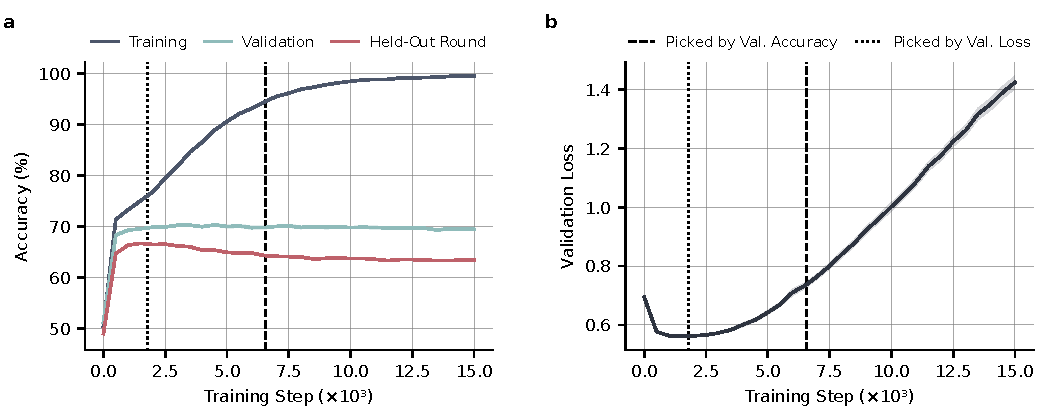
\includegraphics[width=\linewidth]{figures/fig_trajectory.pdf}
\caption{Joint ERM over $15{,}000$ training steps (mean $\pm$ SE over ten seeds, averaged over the four held-out rounds). \textbf{a}, accuracy on the training and validation splits of the training rounds and on the held-out round. \textbf{b}, loss on the same validation splits. Vertical lines mark the average step each selection rule picks.}
\label{fig:trajectory}
\end{figure}

\paragraph{The reported number depends on training length.}
Figure~\ref{fig:selection}a shows what this does to the benchmark number. Selected by validation accuracy, joint ERM scores \num{acc_ERM_val_3000}\% when trained for $3{,}000$ steps and \num{acc_ERM_val_15000}\% when trained for $15{,}000$. Selected by validation loss it scores \num{erm_vloss_range}\% at every length from $1{,}500$ steps up. The paired gain from switching rules is \num{d_rule_15000} points at $15{,}000$ steps and \num{d_rule_3000} at $3{,}000$.

\paragraph{So do method rankings.}
At the benchmark's $15{,}000$ steps and under its selection rule, V-REx, GroupDRO and CORAL beat ERM by \num{d_VREx_ERM_val_15000}, \num{d_GroupDRO_ERM_val_15000} and \num{d_CORAL_ERM_val_15000} points (Figure~\ref{fig:selection}b, Table~\ref{tab:joint}). These are three to four standard errors and would normally be reported as gains. They are not gains in generalization. At the four shorter lengths the same methods and SD are within \num{dg_short_val_absmax} points of ERM, and under validation-loss selection at $15{,}000$ steps they are within \num{dg_long_vloss_absmax}. Their penalties slow the decay that the selection rule fails to catch, which is the job early stopping does for free. IRM is below ERM under either rule.

\begin{figure}[t]
\centering
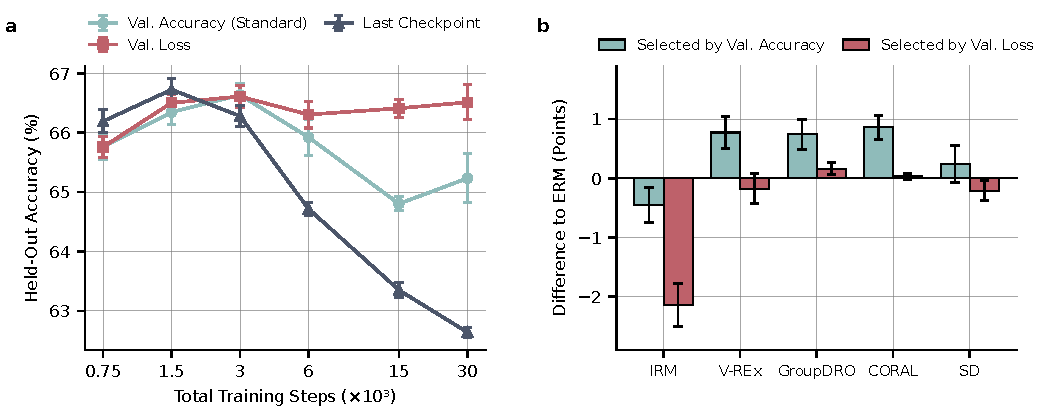
\includegraphics[width=\linewidth]{figures/fig_selection.pdf}
\caption{\textbf{a}, held-out accuracy of joint ERM against training length under three checkpoint-selection rules. \textbf{b}, accuracy of five domain generalization methods minus joint ERM at $15{,}000$ steps, under the two validation rules. Means $\pm$ SE over ten seeds (five at $30{,}000$ steps).}
\label{fig:selection}
\end{figure}

\begin{table}[t]
\centering
\caption{Jointly trained methods: leave-one-round-out test accuracy (\%) at two training lengths under two selection rules, mean $\pm$ SE over ten seeds.}
\label{tab:joint}
\small
\begin{tabular}{lcccc}
\toprule
 & \multicolumn{2}{c}{3{,}000 steps} & \multicolumn{2}{c}{15{,}000 steps} \\
\cmidrule(lr){2-3}\cmidrule(lr){4-5}
Method & Val.\ accuracy & Val.\ loss & Val.\ accuracy & Val.\ loss \\
\midrule
Joint ERM & $66.6\pm0.2$ & $66.6\pm0.2$ & $64.8\pm0.1$ & $66.4\pm0.2$ \\
IRM & $64.9\pm0.3$ & $64.6\pm0.3$ & $64.4\pm0.3$ & $64.3\pm0.3$ \\
V-REx & $67.0\pm0.2$ & $66.6\pm0.1$ & $65.6\pm0.3$ & $66.2\pm0.2$ \\
GroupDRO & $66.9\pm0.1$ & $66.9\pm0.2$ & $65.5\pm0.2$ & $66.6\pm0.2$ \\
CORAL & $66.8\pm0.1$ & $66.6\pm0.2$ & $65.7\pm0.2$ & $66.4\pm0.2$ \\
SD & $66.8\pm0.2$ & $66.4\pm0.2$ & $65.0\pm0.3$ & $66.2\pm0.2$ \\
\bottomrule
\end{tabular}

\end{table}

\paragraph{Learning rate and length are one knob.}
Lowering the learning rate from $5\times10^{-5}$ to $1.5\times10^{-5}$ at $15{,}000$ steps raises ERM by \num{low_gain_val_ERM} points under the standard rule, back to its short-run accuracy. A model trained that way would look like an improved method. Under validation-loss selection the same change is worth \num{low_gain_ERM}.

In the rest of the paper every method is selected by validation loss and reported at all six lengths.

\section{Does PDCL help?}
\label{sec:pdcl}

\subsection{Held-out rounds}

Figure~\ref{fig:budget}a and Table~\ref{tab:seq} give held-out accuracy for joint ERM and the sequential methods. PDCL and fine-tuning are indistinguishable: their paired difference is \num{d_PDCL_RS_Finetune_vloss_1500} at $1{,}500$ steps, \num{d_PDCL_RS_Finetune_vloss_3000} at $3{,}000$, \num{d_PDCL_RS_Finetune_vloss_15000} at $15{,}000$, and never larger than \num{pdcl_ft_absmax} in magnitude (Figure~\ref{fig:budget}b).

Plain replay is worse than no memory. ER is \num{er_ft_range} points below fine-tuning at the four lengths up to $6{,}000$ steps. PDCL is \num{pdcl_er_range} points above ER at those lengths, so dual weighting recovers what replay loses and nothing more. At $15{,}000$ and $30{,}000$ steps all sequential methods have overfit and the differences close.

Sequential training costs \num{ft_erm_range} points against joint ERM at lengths up to $6{,}000$ steps and \num{ft_erm_long_range} at the two longest. Validation loss rescues joint ERM from long training because an early checkpoint is available. It cannot rescue a sequential model, whose early rounds were overfit before the final phase began.

Farthest-first selection changes PDCL by \num{ffpdcl_range} points and ER by \num{ffer_range} across the six lengths. It does not help.

\begin{figure}[t]
\centering
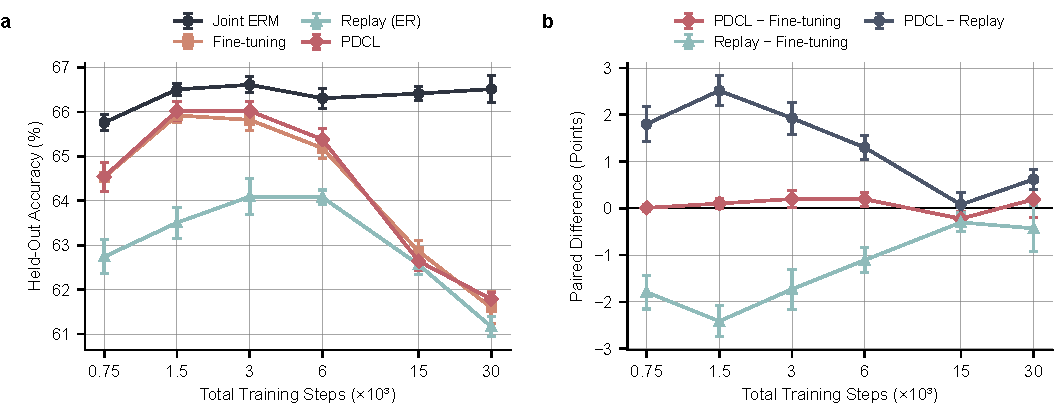
\includegraphics[width=\linewidth]{figures/fig_budget.pdf}
\caption{\textbf{a}, leave-one-round-out test accuracy against total training steps, selected by validation loss. \textbf{b}, paired differences between sequential methods. Means $\pm$ SE over ten seeds (five at $30{,}000$ steps).}
\label{fig:budget}
\end{figure}

\begin{table}[t]
\centering
\caption{Leave-one-round-out test accuracy (\%) by total training steps, selected by validation loss, mean $\pm$ SE over ten seeds (five at $30{,}000$ steps).}
\label{tab:seq}
\small
\begin{tabular}{lcccccc}
\toprule
Method & 750 & 1{,}500 & 3{,}000 & 6{,}000 & 15{,}000 & 30{,}000 \\
\midrule
Joint ERM & $65.8\pm0.2$ & $66.5\pm0.1$ & $66.6\pm0.2$ & $66.3\pm0.2$ & $66.4\pm0.2$ & $66.5\pm0.3$ \\
\midrule
Fine-tuning & $64.5\pm0.3$ & $65.9\pm0.2$ & $65.8\pm0.2$ & $65.2\pm0.2$ & $62.9\pm0.2$ & $61.6\pm0.4$ \\
Replay (ER) & $62.7\pm0.4$ & $63.5\pm0.3$ & $64.1\pm0.4$ & $64.1\pm0.2$ & $62.6\pm0.2$ & $61.2\pm0.2$ \\
ER + FF & $62.6\pm0.3$ & $62.8\pm0.2$ & $63.1\pm0.3$ & $63.7\pm0.2$ & $62.2\pm0.1$ & $61.3\pm0.3$ \\
PDCL & $64.5\pm0.3$ & $66.0\pm0.2$ & $66.0\pm0.2$ & $65.4\pm0.2$ & $62.6\pm0.2$ & $61.8\pm0.2$ \\
PDCL + FF & $64.5\pm0.3$ & $65.7\pm0.3$ & $65.7\pm0.2$ & $65.0\pm0.3$ & $62.4\pm0.2$ & $61.5\pm0.3$ \\
\bottomrule
\end{tabular}

\end{table}

\subsection{Why the memory does not help}
\label{sec:why}

Figure~\ref{fig:mechanism}a shows the loss on the stored examples at the end of training. ER drives it far below the loss on fresh data: \num{mem_ER_3000} at $3{,}000$ steps, where the loss on the validation splits is about $0.6$. Each earlier round holds about 100 stored examples and contributes 32 of them to every step, so a stored example is revisited every three steps while an example of the current round is seen once in 40 to 120. The network memorizes the memory, and held-out accuracy drops.

PDCL holds the same loss at its constraint level: \num{mem_PDCL_RS_3000} against $\epsilon_k=$ \num{eps_PDCL_RS_3000} at $3{,}000$ steps, \num{mem_ratio_3000} times ER's value. It gets there with dual variables that average \num{dual_PDCL_RS_3000} at the end of training, against ER's fixed weight of 1. The constraint on an earlier round is close to satisfied by the model that fine-tuning produces anyway, because fine-tuning forgets only a few points on this benchmark (Section~\ref{sec:retention}). The dual variables therefore stay small, the replay term nearly vanishes from Eq.~\eqref{eq:lagrangian}, and PDCL follows the fine-tuning trajectory. This is Eq.~\eqref{eq:dual} doing what it should.

At long training lengths the picture changes without changing the outcome. The network fits \num{train_PDCL_RS_15000}\% of the current round's training split at \num{val_PDCL_RS_15000}\% validation accuracy (Figure~\ref{fig:mechanism}b), so $\epsilon_k$ is small (\num{eps_PDCL_RS_15000}), the constraints bind, and the dual variables are larger (\num{dual_PDCL_RS_15000}). PDCL then keeps a memorized loss low on a few dozen memorized examples, which says little about accuracy on unseen sequences from that round.

\begin{figure}[t]
\centering
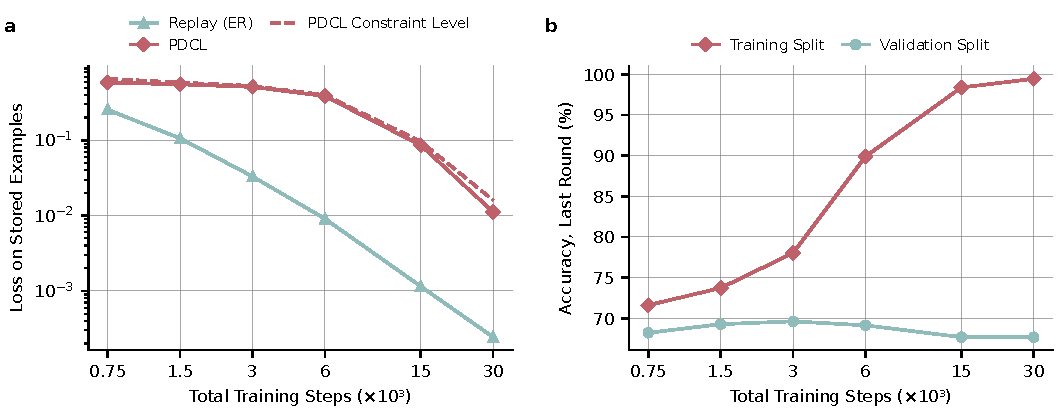
\includegraphics[width=\linewidth]{figures/fig_mechanism.pdf}
\caption{\textbf{a}, loss on the stored examples at the end of training for ER and PDCL, with PDCL's average constraint level $\epsilon_k$. \textbf{b}, PDCL's accuracy on the training and validation splits of the last round at the end of training. Means over ten seeds and four held-out rounds.}
\label{fig:mechanism}
\end{figure}

\subsection{Tuning}
\label{sec:tuning}

Section~\ref{sec:selection} showed that a lower learning rate undoes overfitting, so the fairest long-run comparison uses it. At $15{,}000$ steps and learning rate $1.5\times10^{-5}$ (Figure~\ref{fig:tuning}a, \num{low_n} seeds), fine-tuning gains \num{low_gain_Finetune} points and PDCL \num{low_gain_PDCL_RS}; they end at \num{low_Finetune}\% and \num{low_PDCL_RS}\%, a difference of \num{low_PDCL_RS_Finetune}. ER gains less and is again below fine-tuning (\num{low_ER_Finetune}). The ordering at this setting is the ordering of the short runs. We found the lower rate on seeds 0--4 and the differences held on seeds 5--9.

No PDCL-specific setting changes this (seeds 0--4, $15{,}000$ steps, differences to the default). A dual step size ten times smaller or larger gives \num{var_PDCL_RS_dlr0p001} and \num{var_PDCL_RS_dlr0p1}. A looser constraint, $\epsilon_k$ at twice the training loss, gives \num{var_PDCL_RS_plr5em05_es2}, and a fixed $\epsilon=0.05$ gives \num{var_PDCL_RS_eps0p05}. A memory of $1{,}000$ or $3{,}000$ examples in place of 200 gives \num{var_PDCL_RS_buf1000} and \num{var_PDCL_RS_buf3000} for PDCL and \num{var_ER_buf1000} and \num{var_ER_buf3000} for ER. At $3{,}000$ steps, a lower or a higher learning rate lowers every sequential method.

\subsection{Retention}
\label{sec:retention}

Held-out accuracy is not what continual learning optimizes, so Table~\ref{tab:stream} and Figure~\ref{fig:tuning}b report the four-round stream. Fine-tuning forgets \num{stream_forgetting_Finetune_4000} points at $1{,}000$ steps per round and \num{stream_forgetting_Finetune_20000} at $5{,}000$. That is the whole budget a memory method has to win back. ER wins back part of it at the short length (fine-tuning forgets \num{stream_forget_Finetune_ER_4000} points more) and none at the long one (\num{stream_forget_Finetune_ER_20000}). PDCL sits between the two at the short length and is not separable from either at the long one. Final accuracy over the four rounds is \num{stream_seq_final_range}\% for every sequential method, against \num{stream_final_val_ERM_4000}\% and \num{stream_final_val_ERM_20000}\% for joint ERM.

\begin{figure}[t]
\centering
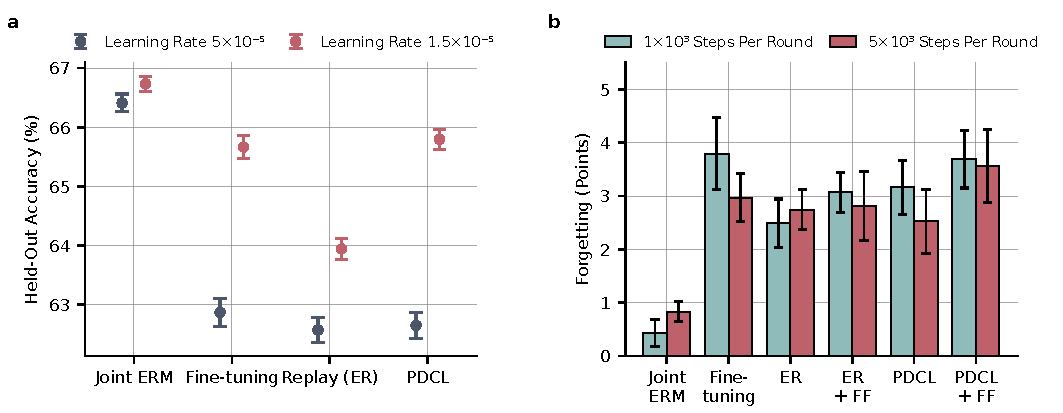
\includegraphics[width=\linewidth]{figures/fig_tuning.pdf}
\caption{\textbf{a}, leave-one-round-out test accuracy at $15{,}000$ steps with the default and a lower learning rate, selected by validation loss. \textbf{b}, forgetting in the four-round stream at two phase lengths. Means $\pm$ SE over seeds.}
\label{fig:tuning}
\end{figure}

\begin{table}[t]
\centering
\caption{Four-round stream: validation accuracy over all four rounds at the end of training (\%) and forgetting (points), mean $\pm$ SE over ten seeds.}
\label{tab:stream}
\small
\begin{tabular}{lcccc}
\toprule
 & \multicolumn{2}{c}{1{,}000 steps per round} & \multicolumn{2}{c}{5{,}000 steps per round} \\
\cmidrule(lr){2-3}\cmidrule(lr){4-5}
Method & Final accuracy & Forgetting & Final accuracy & Forgetting \\
\midrule
Joint ERM & $70.1\pm0.3$ & $0.4\pm0.3$ & $69.2\pm0.3$ & $0.8\pm0.2$ \\
Fine-tuning & $66.5\pm0.6$ & $3.8\pm0.7$ & $65.6\pm0.4$ & $3.0\pm0.4$ \\
Replay (ER) & $66.6\pm0.6$ & $2.5\pm0.5$ & $66.4\pm0.4$ & $2.7\pm0.4$ \\
ER + FF & $65.5\pm0.4$ & $3.1\pm0.4$ & $66.1\pm0.6$ & $2.8\pm0.6$ \\
PDCL & $66.9\pm0.5$ & $3.2\pm0.5$ & $66.4\pm0.4$ & $2.5\pm0.6$ \\
PDCL + FF & $66.5\pm0.4$ & $3.7\pm0.5$ & $65.4\pm0.6$ & $3.6\pm0.7$ \\
\bottomrule
\end{tabular}

\end{table}

\section{Discussion and limitations}

PDCL is useful when earlier tasks are expensive to retain. Here they are cheap: a surrogate fine-tuned on the latest round keeps all but three or four points of accuracy on earlier rounds, and about one point separates it from joint training on a new round. A method that spends effort in proportion to the cost of retention spends almost none, and ends where fine-tuning ends. Replay with fixed weights does worse because it spends the effort regardless and overfits a small memory.

Two consequences follow for this benchmark. When all past rounds can be stored, as they can here, joint retraining with early stopping is the method to beat, and a continual method needs a cost or privacy argument to justify itself. And comparisons selected by validation accuracy should be read with the training length in mind, since a regularizer can look like a better method only because it slows overfitting.

Several things limit these conclusions. All runs use the SeqCNN backbone; a pretrained protein language model may overfit differently. We ran five of the benchmark's domain generalization methods, at default hyperparameters. We adopted validation-loss selection after seeing held-out accuracy decay, so its gain is a diagnosis on this benchmark and should be checked on others; it uses no test data. The labels are computed stability proxies. With four rounds, dual-driven memory allocation makes at most two decisions, and a campaign with many rounds and stronger shifts between them would test PDCL where it has more to do.

\section{Conclusion}

On Antibody DomainBed, primal-dual continual learning matches sequential fine-tuning at every training length and after tuning, and both trail joint training by about a point. Its dual variables correctly report that earlier rounds need little protection, which also explains why fixed-weight replay hurts. Getting to that answer required replacing the benchmark's validation-accuracy rule with validation loss, which removes a dependence on training length large enough to reorder methods. Code and the results of all \num{n_runs} runs are available.

\bibliographystyle{plainnat}
\bibliography{refs}

\end{document}
